%%%%%%%%%%%%%%%%%%%%%%%%%%%%%%%%%%%%%%%%%%%%%%%%%%%%%%%%%%%%%%%%%%%%%%%%%%%%%%%%
%2345678901234567890123456789012345678901234567890123456789012345678901234567890
%        1         2         3         4         5         6         7         8

\documentclass[letterpaper, 10 pt, conference]{ieeeconf}  % Comment this line out
                                                          % if you need a4paper
%\documentclass[a4paper, 10pt, conference]{ieeeconf}      % Use this line for a4
                                                          % paper

\IEEEoverridecommandlockouts                              % This command is only
                                                          % needed if you want to
                                                          % use the \thanks command
\overrideIEEEmargins
% See the \addtolength command later in the file to balance the column lengths
% on the last page of the document

 
% The following packages can be found on http:\\www.ctan.org
%\usepackage{graphics} % for pdf, bitmapped graphics files
%\usepackage{epsfig} % for postscript graphics files
%\usepackage{mathptmx} % assumes new font selection scheme installed
%\usepackage{times} % assumes new font selection scheme installed
%\usepackage{amsmath} % assumes amsmath package installed
%\usepackage{amssymb}  % assumes amsmath package installed
\usepackage[final]{pdfpages}
\usepackage{caption, rotating}
\usepackage{graphics}
\usepackage{array}
\usepackage[export]{adjustbox}
\usepackage[T1]{fontenc}
 
\title{\LARGE \bf
Lowering Depression and Anxiety: A Quantititave Research on the Relationship of Seven Common Habits 
on Human's Mental Health
}
 
\author{Dang Quang Hoang, Karthikeyan Marikrishnan \\ Yuqing Ran, Muhammad Hamza Raza, Hadi Sharifi}



\def\@testdef #1#2#3{%
  \def\reserved@a{#3}\expandafter \ifx \csname #1@#2\endcsname
 \reserved@a  \else
\typeout{^^Jlabel #2 changed:^^J%
\meaning\reserved@a^^J%
\expandafter\meaning\csname #1@#2\endcsname^^J}%
\@tempswatrue \fi}

\begin{document}



\maketitle
\thispagestyle{empty}
\pagestyle{empty}


%%%%%%%%%%%%%%%%%%%%%%%%%%%%%%%%%%%%%%%%%%%%%%%%%%%%%%%%%%%%%%%%%%%%%%%%%%%%%%%%
% \begin{abstract}

% This electronic document is a ÒliveÓ template. The various components of your paper [title, text, heads, etc.] are already defined on the style sheet, as illustrated by the portions given in this document.

% \end{abstract}


%%%%%%%%%%%%%%%%%%%%%%%%%%%%%%%%%%%%%%%%%%%%%%%%%%%%%%%%%%%%%%%%%%%%%%%%%%%%%%%%
\section{INTRODUCTION AND PROBLEM STATEMENT}
Depression and anxiety are two widespread types of disorders that endures a tremendous consequences on
patients themselves, their family, and their society. 
The World Health Organization (WHO) has ranked depression as the fourth leading cause of human disability 
and by 2020, it reaches to second leading cause \cite{kessler2013epidemiology}. It is well known that depression causes health 
degradation \cite{verma2017impact} and directly causes cardiovascular diseases \cite{bradley2015depression}. 
A recent study in 2017 showed that depression 
increases the risk of cardiovascular by 80\% \cite{penninx2017depression}. In case of anxiety, in average, up to 33.7\% of 
the human populations expereinces anxiety \cite{bandelow2015epidemiology} in their life time. Anxiety's affects go beyond physical
and it causes learning and reasoning incapacities \cite{spielberger2013effects}\cite{darke1988effects}. 
This proposal analyzes data from the Behavioral Risk Factor Surveillance System (BRFSS), collected in several years. 
It tries to find a relationship between six habit factors (physical activity, binge eating disorder, 
smoking, drinking alcohol, and social media/technology) and depression and anxiety. It proposes a
solutions that could lead to reduction of depression and anxiety in the society. 

\section{OBJECTIVE}

\noindent\textit{$\circ$ What this research is trying to accomplish?} \newline
\textnormal{
Identifying the relation between the six factors and depression and anxiety. 
And provide guidelines based on the six factors to reduce depression and anxiety in the human life.
}

\setlength{\parskip}{1em} %give space between paragraph. Except for the first one above.

\par\noindent\textit{$\circ$ How is research in this field is done today; what are the limits of current practice?}\newline
\textnormal{
Currently, research papers in human disorder, analyzes few habit factors 
and mainly focused on depression or anxiety. (Hadi: more to be written) 
}
\par\noindent\textit{$\circ$ What's new to this research? Why will it be successful?}\newline
\textnormal{
This proposal touches more comprehensive number of habits and the outcome of the 
research provides guidance for larger body of human society. The key to success 
of this research is data and linking data to the right conclusion. Thanks to the 
BRFSS data and many researches done in this field, this research will reach to a 
scientific conclusion that provide guidelines for society to avoid or reduce 
depression and anxiety. That is the success of this research.
}
\par\noindent\textit{$\circ$ Who cares?}\newline
\textnormal{
The general public, medical society, insurance industry, and corporation. Depression 
and anxiety are felt in each and every part of the human life and it is in interest 
of all above mentioned to control or reduce outcome of anxiety and depression affect.
}
\par\noindent\textit{$\circ$ If this research is successful, what difference and impact will it make, and how do you measure them?}\newline
\textnormal{
The success of this research will provide guidelines for different sectors of 
human society to avoid anxiety and depression and identify them at the early 
stage of disease. It will provide recipes to various human resource organization 
on how to avoid anxiety and depression. Surveys such BRFSS and local and internal 
surveys can provide a great measure on how this research impacted them.
}
\par\noindent\textit{$\circ$ What are the risks and payoffs?}\newline
\textnormal{
The risk is to convince mass public, human resource organizations, and small 
to large companies that the results of this research will indeed assist them 
get better and faster results. The payoffs is happier work, happier life, 
happier families, and happier society.  
}
\par\noindent\textit{$\circ$ How much will it cost?}\newline
\textnormal{
The biggest cost is the time. The data is available, but it 
needs to be cleaned, the related information to be extracted, and analyzed. 
The research, at this preliminary stage, anticipates 150 to 200 hours of scientific work. 
}
\par\noindent\textit{$\circ$ How long will it take?}\newline
\textnormal{
The proposal touches the tip of the ice of controlling and identifies anxiety 
and depression. This research starts with what data is currently available 
and pave the path to larger research in the field of mental disease. This 
proposal can be done in one to two quarter of a year.
}
\par\noindent\textit{$\circ$ How will progress be measured.}\newline
\textnormal{
The progress of this research is measured by first establishing a clear connection 
between the six habits and anxiety and depression. Second understanding how these 
factors can decrease anxiety and depression. And third provides the golden 
guidelines for various parties.
}
\section{LITERATUR REVIEW}

\section{METHODLOGY}
The research requires analyzing large data that are not clean and not organized in 
a traditional database concept we are familiar with. The main task of our team is 
extract data from the assigned topic, clean the data, put it a format that all 
other teammates will agree upon. From that point, we analyze the data and drive 
conclusions. Our conclusion will be the blue print for the guidelines we will prepare 
as the outcome of this research. 
Figure \ref{fig:schedule} shows the details on how various tasks are distributed among team members 
and how the timeline is formed to reach all the deadlines. 

%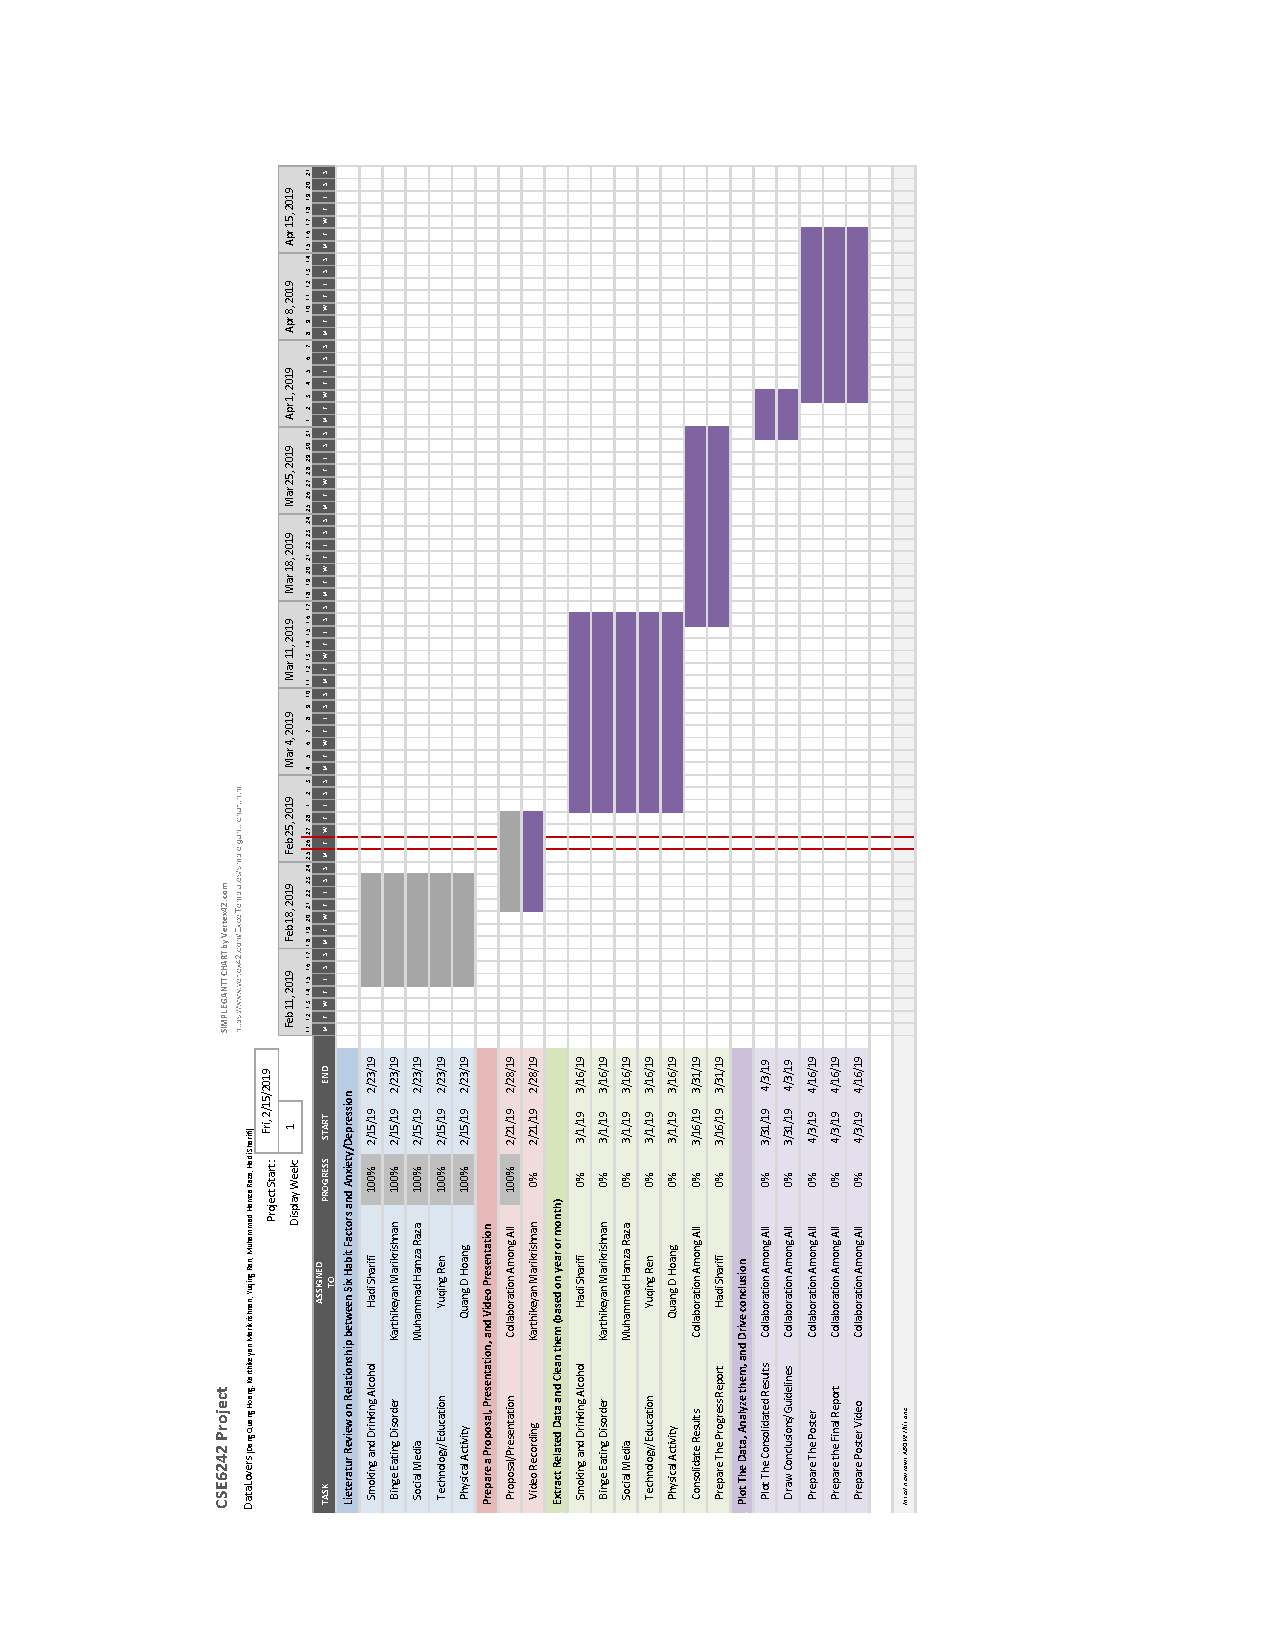
\includepdf{schedule.pdf}
%\captionsetup[figure]{labelformat=empty}
\clearpage 
\begin{figure}[hbt!]
        \centering
        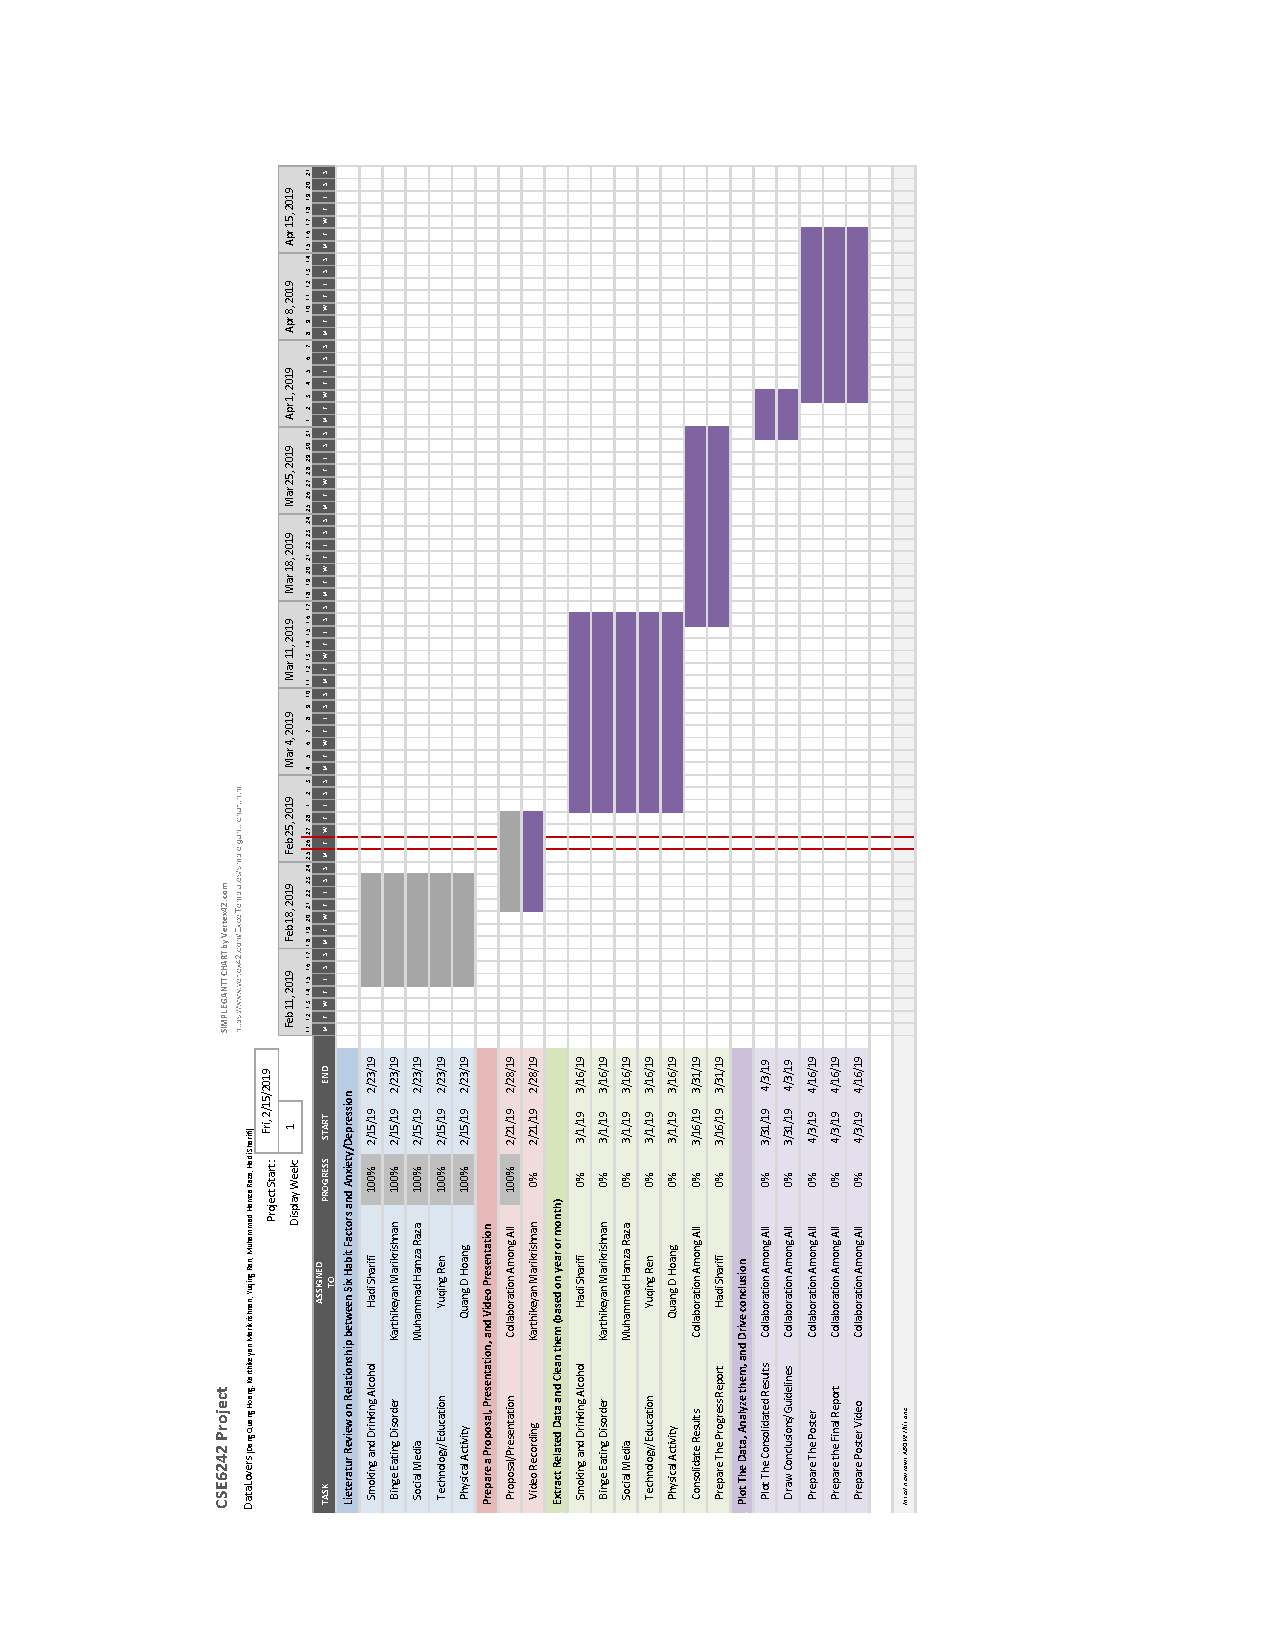
\includepdf[pages=-]{schedule.pdf}
        \addvspace{250pt}
        
        \hspace{-10cm}
        \rotatebox{90}{ Figure ~\ref{fig:schedule}: The schedule of the team for the research.}
        
        %\caption{The Schedule of all tasks defined for the team.}
        \caption{}
        \label{fig:schedule}
\end{figure}

\clearpage 


\bibliography{biblio}
\bibliographystyle{plain}

\end{document}
